% move all configuration stuff into one file so we can focus on the content
\documentclass[aspectratio=169,hyperref={pdfpagelabels=false,colorlinks=true,linkcolor=white,urlcolor=blue},t]{beamer}

%%%%%%%%%%%%%%%%%%%%%%%%%%%%%%%%%%%%%%%%%%%%%%%%%%%%%%%%%%%%%%%%%%%%%%%%%%%%%%%%%%
%%%%%%%%%%%%%%%%%%%%%%%%%%%%%%%%%%%%%%%%%%%%%%%%%%%%%%%%%%%%%%%%%%%%%%%%%%%%%%%%%%
% packages
\usepackage{pict2e}
\usepackage{epic}
\usepackage{amsmath,amsfonts,amssymb}
\usepackage{units}
\usepackage{fancybox}
\usepackage[absolute,overlay]{textpos} 
\usepackage{media9} % avi2flv: "C:\Program Files\ffmpeg\bin\ffmpeg.exe" -i TuneFreqFilterbank.avi -b 600k -s 441x324 -r 15 -acodec copy TuneFreqFilterbank.flv
\usepackage{animate}
\usepackage{gensymb}
\usepackage{multirow}
\usepackage{silence}
\usepackage[backend=bibtex,style=ieee]{biblatex}
\AtEveryCitekey{\iffootnote{\tiny}{}}
\addbibresource{references}

%%%%%%%%%%%%%%%%%%%%%%%%%%%%%%%%%%%%%%%%%%%%%%%%%%%%%%%%%%%%%%%%%%%%%%%%%%%%%%%%%%
%%%%%%%%%%%%%%%%%%%%%%%%%%%%%%%%%%%%%%%%%%%%%%%%%%%%%%%%%%%%%%%%%%%%%%%%%%%%%%%%%%
% relative paths
\graphicspath{{graph/}}


%%%%%%%%%%%%%%%%%%%%%%%%%%%%%%%%%%%%%%%%%%%%%%%%%%%%%%%%%%%%%%%%%%%%%%%%%%%%%%%%%%
%%%%%%%%%%%%%%%%%%%%%%%%%%%%%%%%%%%%%%%%%%%%%%%%%%%%%%%%%%%%%%%%%%%%%%%%%%%%%%%%%%
% units
\setlength{\unitlength}{1mm}

%%%%%%%%%%%%%%%%%%%%%%%%%%%%%%%%%%%%%%%%%%%%%%%%%%%%%%%%%%%%%%%%%%%%%%%%%%%%%%%%%%
%%%%%%%%%%%%%%%%%%%%%%%%%%%%%%%%%%%%%%%%%%%%%%%%%%%%%%%%%%%%%%%%%%%%%%%%%%%%%%%%%%
% theme & layout
\usetheme{Frankfurt}
\beamertemplatenavigationsymbolsempty
%\setbeamertemplate{frametitle}[smoothbars theme]
\setbeamertemplate{frametitle}
{
    \begin{beamercolorbox}[ht=1.8em,wd=\paperwidth]{frametitle}
        \vspace{-.1em}%
        \hspace{.2em}{\strut\insertframetitle\strut}
        
        \hspace{.2em}\small\strut\insertframesubtitle\strut
        %\hfill
        %
\includegraphics[height=.8cm,keepaspectratio]{CenterMusicTechnology-solid-2lines-white-CoAtag}
        
    \end{beamercolorbox}
    \begin{textblock*}{100mm}(11.6cm,.7cm)
        \includegraphics[height=.8cm,keepaspectratio]{logo_GTCMT_black}
    \end{textblock*}
}

% set this to ensure bulletpoints without subsections
\usepackage{remreset}
\makeatletter
\@removefromreset{subsection}{section}
\makeatother
\setcounter{subsection}{1}

%---------------------------------------------------------------------------------
% appearance
\setbeamercolor{structure}{fg=gtgold}
\setbeamercovered{transparent} %invisible
\setbeamercolor{bibliography entry author}{fg=black}
\setbeamercolor*{bibliography entry title}{fg=black}
\setbeamercolor*{bibliography entry note}{fg=black}

%\usepackage{pgfpages}
%\setbeameroption{show notes}
%\setbeameroption{show notes on second screen=right}
%---------------------------------------------------------------------------------
% fontsize
\let\Tiny=\tiny

%%%%%%%%%%%%%%%%%%%%%%%%%%%%%%%%%%%%%%%%%%%%%%%%%%%%%%%%%%%%%%%%%%%%%%%%%%%%%%%%%%
%%%%%%%%%%%%%%%%%%%%%%%%%%%%%%%%%%%%%%%%%%%%%%%%%%%%%%%%%%%%%%%%%%%%%%%%%%%%%%%%%%
% warnings
\pdfsuppresswarningpagegroup=1
\WarningFilter{biblatex}{Patching footnotes failed}
\WarningFilter{latexfont}{Font shape}
\WarningFilter{latexfont}{Some font shapes}
\WarningFilter{gensymb}{Not defining}



\subtitle{Part 3.1: Fundamentals I}

%%%%%%%%%%%%%%%%%%%%%%%%%%%%%%%%%%%%%%%%%%%%%%%%%%%%%%%%%%%%%%%%%%%%%%%%%%%%
\begin{document}
    % generate title page
	

\begin{frame}
    \titlepage
    %\vspace{-5mm}
    \begin{flushright}
        \href{http://www.gtcmt.gatech.edu}{\includegraphics[height=.8cm,keepaspectratio]{logo_GTCMT_black}}
    \end{flushright}
\end{frame}


    \section[overview]{lecture overview}
        \begin{frame}{introduction}{overview}
            \begin{itemize}
                \item   \textbf{text book}  
                    \begin{itemize}
                        \item   \href{http://ieeexplore.ieee.org/xpl/ebooks/bookPdfWithBanner.jsp?fileName=6331119.pdf&bkn=6266785&pdfType=chapter}{\underline{\textit{Chapter 2: Fundamentals} (pp.~7--20)}}
                    \end{itemize}
                \item   \textbf{additional reading}  
                    \begin{itemize}
                        \item   Richard G.~Lyons, \textit{Understanding Digial Signal Processing}, 3rd, Prentice Hall/Pearson, 2011
                    \end{itemize}
                \bigskip
                \item<2->   \textbf{lecture content}
                    \begin{itemize}
                        \item<2->   periodic and random signals
                        \item<3->   sampling and quantization
                        \item<4->   statistical signal description
                        \item<5->   convolution
                        \item<6->   block-based processing
                    \end{itemize}
            \end{itemize}
        \end{frame}
        
    \section[intro]{introduction}
        \begin{frame}\frametitle{audio signals}\framesubtitle{signal categories}
            \begin{itemize}
                \item	\textbf{deterministic signals}:\\
                        \textit{predictable}: future shape of the signal can be known (example: sinusoidal)
                \pause		
                \item	\textbf{random signals}:\\
                        \textit{unpredictable}: no knowledge can help to predict what is coming next (example: white noise)
            \end{itemize}
            
            \bigskip
            \pause
            ``real-world'' audio signals can be modeled as time-variant combination of 
            \begin{itemize}
                \item	(quasi-)periodic parts
                \item	(quasi-)random parts
            \end{itemize}
        \end{frame}

    \section[periodic]{periodic signals}
        \begin{frame}{audio signals}{periodic signals 1/4}
            \setbeamercovered{invisible}

            periodic signals: most prominent examples of deterministic signals
            \begin{eqnarray*}
                x(t) 	&=& x(t+T_0)\\
                f_0 	&=& \frac{1}{T_0} =  \frac{\omega_0}{2\pi}
            \end{eqnarray*}
            \vspace{-9mm}

            \visible<2>{
                \begin{figure}
                    \centering
                    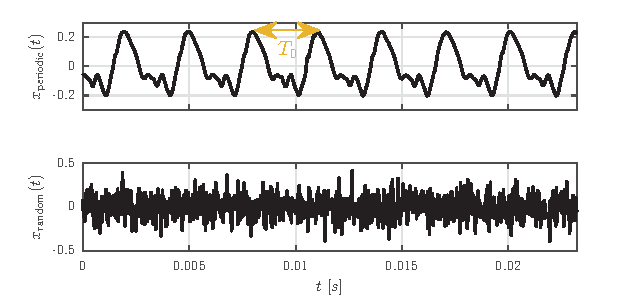
\includegraphics{PeriodicRandom}
                \end{figure}
                \only<2>{
                \begin{textblock*}{\baselineskip }(1.1\textwidth,.5\textheight)
                    \rotatebox{90}{\tiny matlab source: matlab/displayPeriodicRandom.m}
                \end{textblock*}}
            }
        \end{frame}

        \begin{frame}{audio signals}{periodic signals 2/4}
            periodic signal $\Rightarrow$ representation in \textbf{Fourier series}
            \begin {equation}
                x(t) = \sum\limits_{k=-\infty}^{\infty} {\color<5>{gtgold}{a_k}} {\color<4>{gtgold}{\e^{\mathrm{j}{\color<2-3>{gtgold}{\omega_0}} {\color<3>{gtgold}{k}} t}}} \nonumber
            \end {equation}
            \begin{itemize}
                \item<2-> $\omega_0 = 2\pi\cdot f_0$
                \item<3-> $k\omega_0$: integer multiples of the lowest frequency
                \item<4-> $\e^{\jom_0kt} = \cos(\omega_0kt) + \mathrm{j} \sin(\omega_0kt)$
                \item<5-> $a_k$: Fourier coefficients --- amplitude of each component
                    \begin {equation}\label{eq:fourier_coeff}
                        a_k = \frac{1}{T_0}\int\limits_{-\nicefrac{T_0}{2}}^{\nicefrac{T_0}{2}} x(t) \e^{-\jom_0kt}\, dt \nonumber
                    \end {equation}
            \end{itemize}
        \end{frame}

        \begin{frame}{audio signals}{periodic signals 2/4}
            \toremember{}
            
            \begin{block}{Fourier Series}
                \begin{itemize}
                    \item   \textbf{every} periodic signal can be represented in a Fourier series
                    \item   a periodic signal \textbf{contains only} frequencies at integer multiples of the fundamental frequency $f_0$
                    \bigskip
                    \item<2->   Fourier series can only be applied to periodic signals
                    \item<2->   Fourier series is analytically elegant but only of limited practical use as the fundamental period has to be known
                \end{itemize}
            \end{block}
        \end{frame}

        \begin{frame}{audio signals}{periodic signals 3/4}
            reconstruction of periodic signals with limited number of sinusoidals:
            \begin {equation*}
                \hat{x}(t) = \sum\limits_{k=-\mathcal{K}}^{\mathcal{K}} a_k e^{\jom_0kt}
            \end {equation*}
            %\vspace{-5mm}
            \only<1>{
                \begin{figure}
                    \centering
                    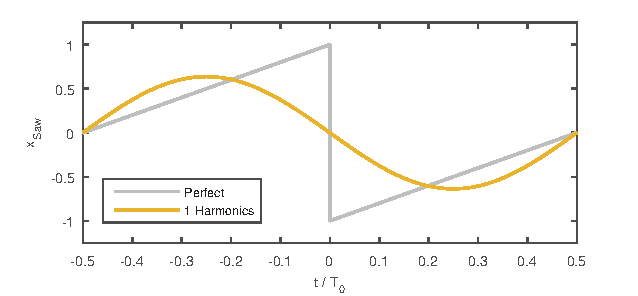
\includegraphics{graph/AdditiveSynthesisSaw-1}
                \end{figure}
                \begin{textblock*}{\baselineskip }(1.1\textwidth,.5\textheight)
                    \rotatebox{90}{\tiny matlab source: matlab/displayAdditiveSynthesis.m}
                \end{textblock*}
            }
            
            \setcounter{i}{1}
            \whiledo{\value{i}<6}	
            {
                \pause
                \only<\value{beamerpauses}>
                {
                    \begin{figure}
                        \centering
                        \includegraphics{graph/AdditiveSynthesisSaw-\arabic{i}}
                    \end{figure}
                    \audioautoplay{audio/additivesynthesis_saw_\arabic{i}.mp3}
                    
                    \begin{textblock*}{\baselineskip }(1.1\textwidth,.5\textheight)
                        \rotatebox{90}{\tiny matlab source: matlab/displayAdditiveSynthesis.m}
                    \end{textblock*}
                }
                \stepcounter{i} 
            }	
            
            \setcounter{i}{1}
            \whiledo{\value{i}<6}	
            {
                \pause
                \only<\value{beamerpauses}>
                {
                    \begin{figure}
                        \centering
                        \includegraphics{graph/AdditiveSynthesisRect-\arabic{i}.pdf}
                    \end{figure}
                    \audioautoplay{audio/additivesynthesis_rect_\arabic{i}.mp3}
                    
                    \begin{textblock*}{\baselineskip }(1.1\textwidth,.5\textheight)
                        \rotatebox{90}{\tiny matlab source: matlab/displayAdditiveSynthesis.m}
                    \end{textblock*}
                }
                \stepcounter{i} 
            }	
        \end{frame}

    \section[random]{random signals}
%\begin{frame}{audio signals}{random process}
	%\textbf{random process}: ensemble of random series
	%\begin{figure}
		%\centering
			%\includegraphics[scale=.25]{graph/randomprocess}
	%\end{figure}
	%\pause
	%special cases:
	%\begin{itemize}
		%\item	\textbf{stationarity}: all parameters (such as the mean) are time invariant
		%\item	\textbf{ergodicity}: process with equal time and ensemble mean (implies stationarity)
	%\end{itemize}
%\end{frame}
	%
%\subsection{sampling \& quantization}
	%\begin{frame}\frametitle{digital signals}\framesubtitle{introduction}
		%digital signals can only be represented with a limited number of values
		%\pause
		%
		%$\Rightarrow$
		%\begin{itemize}
			%\item	time discretization: \textbf{sampling}
			%\item	amplitude discretization: \textbf{quantization}
		%\end{itemize}
	%\end{frame}
	%
	%\begin{frame}\frametitle{digital signals}\framesubtitle{sampling}
		%\begin{equation}
			%T_{\mathrm{S}} = \frac{1}{f_{\mathrm{S}}} 
		%\end{equation}
		%\begin{figure}
			%\centering
				%\includegraphics[scale=.6]{\AcaGraph/sampling}
			%\label{fig:sampling}
		%\end{figure}
		%\pause
		%typical sample rates
		%\begin{itemize}
			%\item	\unit[8--16]{kHz}: speech (phone)
			%\item	\unit[44.1--48]{kHz}: (consumer) audio/music
			%\item	higher: production audio
		%\end{itemize}
	%\end{frame}	
	%
	%\begin{frame}\frametitle{digital signals}\framesubtitle{sampling ambiguity 1/2}
		%\begin{eqnarray}
			%f_0 &=& \unit[1, 5, 7]{kHz}\\
			%f_{\mathrm{S}} &=& \unit[6]{kHz}
		%\end{eqnarray}
		%\begin{figure}
			%\centering
				%\includegraphics[scale=.7]{\AcaGraph/samplingambig}
				%\label{fig:samplingambig}
		%\end{figure}
	%\end{frame}	
	%
	%\begin{frame}\frametitle{sampling and quantization}\framesubtitle{sampling ambiguity 2/2}
		%\textbf{wagon wheel effect}
		%\invisible<2->{
		%\begin{figure}
			%\begin{center}
				%\includegraphics[scale=.4]{graph/Stagecoach-Western}
			%\end{center}
		%\end{figure}
		%}
		%\visible<2->{
			%\vspace{-60mm}
			%\begin{figure}
				%\begin{center}
					%\includegraphics[scale=.2]{graph/Stagecoach-Western}
				%\end{center}
			%\end{figure}
			%\begin{enumerate}
				%\item	$f_{wheel} < \frac{f_S}{2}$: speeding up
				%\pause
				%\item	$\frac{f_S}{2} < f_{wheel} < f_S$: slowing down
				%\pause
				%\item	$f_{wheel} = f_S$: standing still
				%\pause
				%\item	$\ldots$
			%\end{enumerate}
		%}
	%\end{frame}
	%
	%\begin{frame}\frametitle{digital signals}\framesubtitle{sampling theorem 1/2}
		%\vspace{-10mm}
		%\begin{flushright}
			 %\includegraphics[scale=.25]{Graph/exclamation-mark}
		%\end{flushright}
		%\begin{block}{sampling theorem}
			%\centering
			%A sampled signal can  be reconstructed without loss of information if the sample rate $f_{\mathrm{S}}$ is higher than twice the bandwidth $f_{\mathrm{max}}$  in the sampled audio signal.
			%\begin{equation}\label{eq:sample_theorem}	
				%f_{\mathrm{S}} > 2\cdot f_{\mathrm{max}}
			%\end{equation}
		%\end{block}
	%\end{frame}	
	%
	%\begin{frame}\frametitle{digital signals}\framesubtitle{sampling theorem: aliasing 2/2}
		%\begin{figure}
			%\centering
				%\includegraphics[scale=.7]{\AcaGraph/spectral_overlap}
		%\end{figure}
	%\end{frame}	
	%
	%\begin{frame}\frametitle{digital signals}\framesubtitle{quantization}
		%continuous amplitude values are rounded to pre-defined set of allowed amplitude values
		%\begin{figure}
			%\centering
				%\includegraphics[scale=.7]{\AcaGraph/quant}
		%\end{figure}
        %\vspace{-3mm}
		%\pause
		%\begin{itemize}
			%\item	\textbf{number of quantization steps}: $\mathcal{M} = 16$
			%\item	\textbf{word length}: $w = \log_2(\mathcal{M}) = \unit[4]{bit}$
		%\end{itemize}
	%\end{frame}	
%
	%\begin{frame}\frametitle{digital signals}\framesubtitle{quantization: number of quantization steps}
		%\begin{table}
			%\centering
			%\begin{tabular}{lcr}
			%\hline
				%$w$ & $\mathcal{M} = 2^w$ \\
			%\hline
				%1	&	2\\
				%2	&	4\\
				%4	&	16\\
				%8	&	256\\
				%12	&	4096\\
				%16	&	65536\\
				%20	&	1048576\\
				%24	&	16777216\\
			%\end{tabular}  
		%\end{table}
	%\end{frame}	
%
	%\begin{frame}\frametitle{digital signals}\framesubtitle{quantization: process}
		%\begin{figure}
			%\centering
			 %\includegraphics[scale=0.13]{Graph/Flowchart_Quantization}
		%\end{figure}
		%\begin{equation}
			%e_{\mathrm{Q}}(i) = x(i) - x_{\mathrm{Q}}(i)
		%\end{equation}
	%\end{frame}	
	%
	%%\begin{frame}\frametitle{digital signals}\framesubtitle{quantization: SNR 1/2}
		%%\vspace{-5mm}
		%%\begin{columns}[lr]
			%%\column{6cm}
			%%What is the SNR of a quantized sinusoidal?
			%%\begin{equation}\label{eq:snr}
				%%SNR = 10\cdot\log_{10}\left(\frac{W_{\mathrm{S}}}{W_{\mathrm{Q}}}\right)\; [dB] 
			%%\end{equation}
			%%
			%%\hspace{3mm}use: $sin^2(t) = \frac{1-cos(2t)}{2}$
			%%
			%%\column{4cm}
			%%%\hspace{5mm}
			%%\begin{flushright}
				 %%\includegraphics[scale=.08]{Graph/question-mark}
			%%\end{flushright}
		%%\end{columns}
		%%
		%%\pause
		%%\begin{eqnarray}
			%%W_S &=& \frac{A^2}{2} = \frac{(\Delta\cdot 2^{w-1})^2}{2}\\
			%%W_Q &=& \frac{\Delta^2}{12}\\
			%%\pause
			%%\frac{W_S}{W_Q} &=& \frac{3}{2}\cdot 2^{2w}
		%%\end{eqnarray}
	%%\end{frame}		
	%\begin{frame}\frametitle{digital signals}\framesubtitle{quantization: SNR}
		%\begin{block}{Signal-to-Noise Ratio}
			%\centering
			%\begin{equation}
				%SNR = 6.02\cdot w + c_{\mathrm{S}}\quad [dB]
			%\end{equation}
			%\begin{itemize}
				%\item	every additional bit adds app.\ \unit[6]{dB} SNR
				%\item	constant $c_{\mathrm{S}}$ depends on signal (scaling and PDF)
			%\end{itemize}
		%\end{block}
		%\pause
		%\begin{itemize}
			%\item	square wave (full scale): $c_{\mathrm{S}} =  \unit[10.80]{dB}$
			%\item	sinusoidal wave (full scale): $c_{\mathrm{S}} =  \unit[1.76]{dB}$
			%\item	rectangular {PDF} (full scale): $c_{\mathrm{S}} =  \unit[0]{dB}$
			%\item	Gaussian {PDF} (full scale = $4\sigma_{g}$): $c_{\mathrm{S}} =  \unit[-7.27]{dB}$
		%\end{itemize}
	%\end{frame}		
	%
	%\begin{frame}\frametitle{digital signals}\framesubtitle{amplitude in DSP}
		%floating point: $x_{\mathrm{Q}} = M_{\mathrm{G}}\cdot 2^{E_{\mathrm{G}}}$
		%\begin{figure}
			%\centering
			 %\includegraphics[scale=.3]{Graph/floatingpoint}
		%\end{figure}
		%\begin{itemize}
			%\item	signal amplitude: $-1 \leq x_{\mathrm{Q}} < 1$\\
			%\item	level: max.\ amplitude $\mapsto \unit{0}{dBFS}$
		%\end{itemize}
	%\end{frame}
	%
	%\begin{frame}\frametitle{statistical signal description}\framesubtitle{probability density function}
		%PDF $p_x(x)$
		%\begin{itemize}
			%\item	abscissa: possible (amplitude) values
			%\item	ordinate: probability
		%\end{itemize}
		%\pause
		%\begin{eqnarray}
			%p_x(x)&\geq& 0 , and\\	
			%\int\limits_{-\infty}^{\infty}{p_x(x)\, dx} &=& 1	
		%\end{eqnarray}
		%\pause
		%RFD (Approximation)
		%\begin{itemize}
			%\item[] histogram of (amplitude) values
		%\end{itemize}
	%\end{frame}	
		%
	%\begin{frame}\frametitle{statistical signal description}\framesubtitle{PDF: examples 1/2}
		%\only<1>
		%{
			%\begin{flushright}
				 %\includegraphics[scale=.08]{Graph/question-mark}
			%\end{flushright}
			%\vspace{-3mm}
			%PDF shape for:
			%\begin{itemize}
				%\item	square wave
				%\item	sawtooth wave
				%\item	sine wave
				%\item	white noise (uniform, gaussian)
				%\item	DC
			%\end{itemize}
		%}
		%\uncover<2->
		%{
			%\begin{figure}
				%\centering
				 %\includegraphics[scale=.7]{\AcaGraph/pdfs}
			%\end{figure}
		%}
	%\end{frame}	
		%
	%\begin{frame}\frametitle{statistical signal description}\framesubtitle{PDF: real world signals 2/2}
		%\begin{figure}
			%\centering
			 %\includegraphics[scale=.7]{\AcaGraph/realpdf}
		%\end{figure}
	%\end{frame}	
    
    \section[summary]{lecture summary}

\end{document}

